\chapterauthor{Karl Thyssen}
Here we will discuss the results we saw for the various approaches we attempted.

As previously mentioned we experimented with a $\gamma$ value of $1.0$ and $0.9$ after which we continued other variations at $\gamma = 0.9$.
Other variations include:
\begin{itemize}
	\item $\gamma = 1.0$:
	\begin{itemize}
		\item Generation 0 data generated from 4 $\code{simple\_agents}$
		\begin{itemize}
			\item Additionally train MLB
		\end{itemize}
	\end{itemize}
	\item $\gamma = 0.9$:
	\begin{itemize}
		\item Generation 0 data generated from 4 $\code{simple\_agents}$:
		\begin{itemize}
			\item self-train until agents begin to regularly interact with each other
			\item self-train
			\item state vector reduced to 180 elements
		\end{itemize}
		\item Generation 0 data generated from 4 $\code{random\_agents}$:
		\begin{itemize}
			\item self-train until agents begin to regularly interact with each other
			\item self-train
		\end{itemize}
	\end{itemize}
\end{itemize}

%Discuss reasons behind initial approach - also mlp regressor (slow to fit so less data)
\subsection{The initial approach}

Having decided on the random forest regressors as the medium for storing our Q, and knowing the random forest has the ability to determine feature importances and weightings itself we decided to throw every feature we could think at it as described in \ref{State_rep}. We initially also chose a $\gamma$ value of $1.0$ for simplicity in testing and began to train an agent. In \cite{paper} the agent trains for 10000 episodes per generation and begins to show a large improvement between generations $10$ and $20$, however that agent is trained using a neural network so we expected a longer wait before seeing such spikes in performance. This is due to the erratic nature of the predictions made by the forests in relation to the MLP we tested.

Out of interest we also tested the same set-up using an MLP regressor, however unlike the forest, the impact of using any and all features was an exorbitant time required for the fitting after each generation, often longer than the data generation itself.

The average time required to generate data for and fit each generation was roughly $4800 seconds$. This time required is clearly dependent not only on hardware and thinking time but also the number of steps the agent takes per episode which was unfortunately consistently short.

\begin{figure}[h]
\centering
	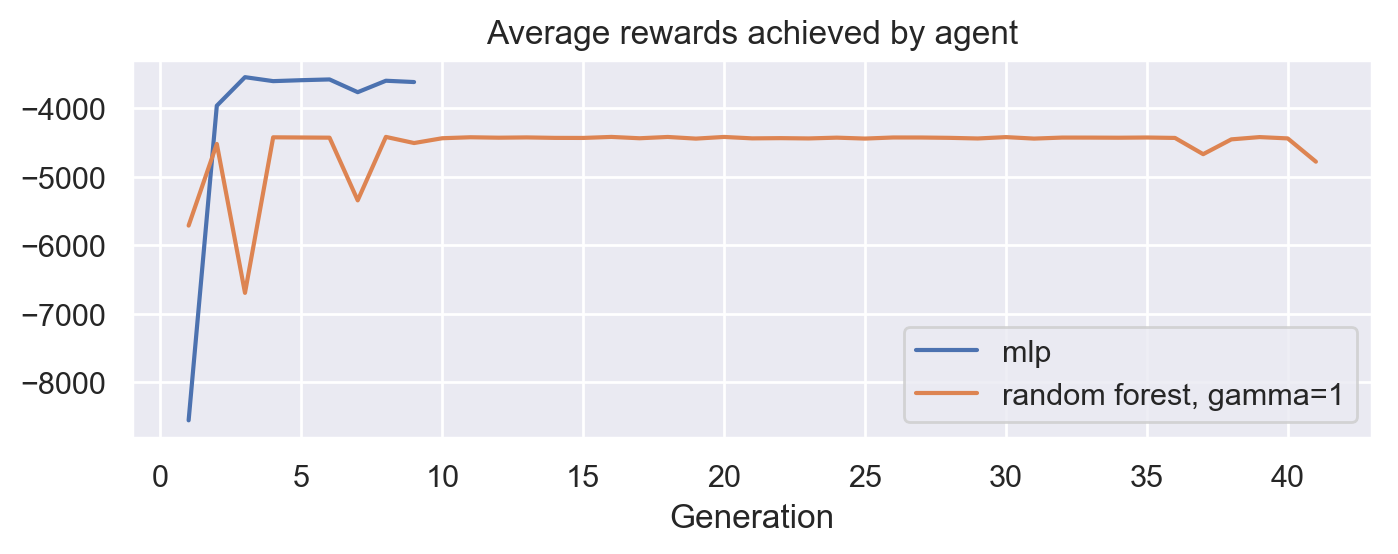
\includegraphics[width=\linewidth]{images/mlp_vs_forest_gamma_1.png}
	\caption{Here we see the performance of 40 generations trained with the random forest and 8 generations using the MLP. We chose not to train the MLP further as the time constraints were too severe and we were not seeing any improvement.}
	\label{mlp_vs_forest_gamma_1.0}
\end{figure}


%show results of initial training
%random forest too erratic - as single steps can be fatal, inaccuracies can have drastic consequences
%let train for a long time as unclear when we should see results
%present variations
%discuss changes and possible solutions - even fewer features, other machine learning methods

